\subsection{Моделирование механических процессов, проетекающих в электронном модуле и устройстве в целом}

Результаты частотного анализа в \textit{SOLIDWORKS Simulation} первого варианта компоновки ПП представлены на рисунке 8.

\begin{figure}[H]
  \centering
  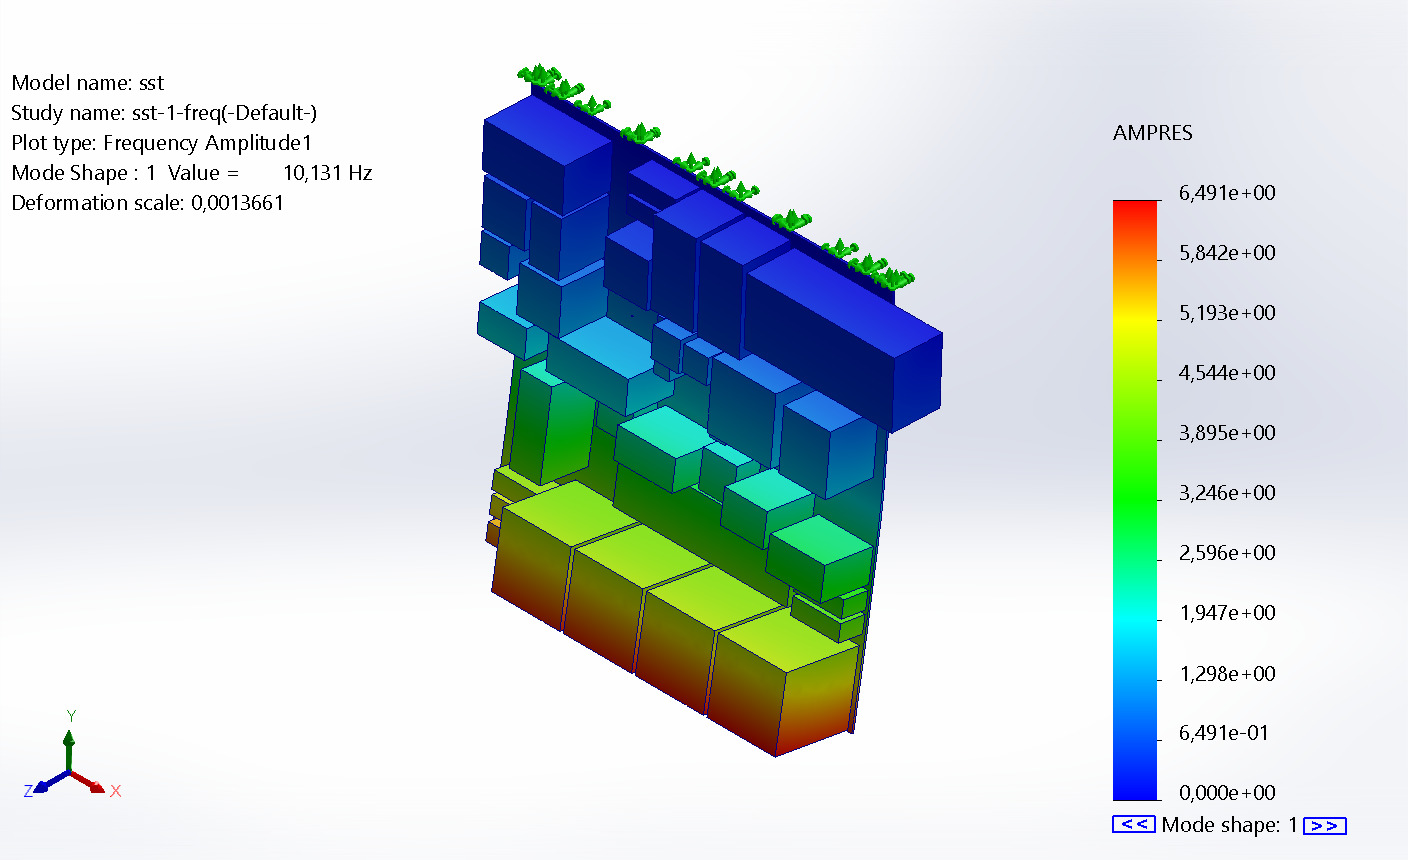
\includegraphics[scale=0.3]{../img/sst-1/freq/top_view/sst-sst-1-freq-Amplitude-Amplitude1.jpg}
  \caption{Результаты частотного анализа в \textit{SOLIDWORKS SIMULATION} первого варианта компоновки ПП.}
\end{figure}


На рисунке 9 представлены результаты частотного анализа в \textit{SOLIDWORKS Simulation} второго варианта компоновки печатной платы.

\begin{figure}[H]
  \centering
  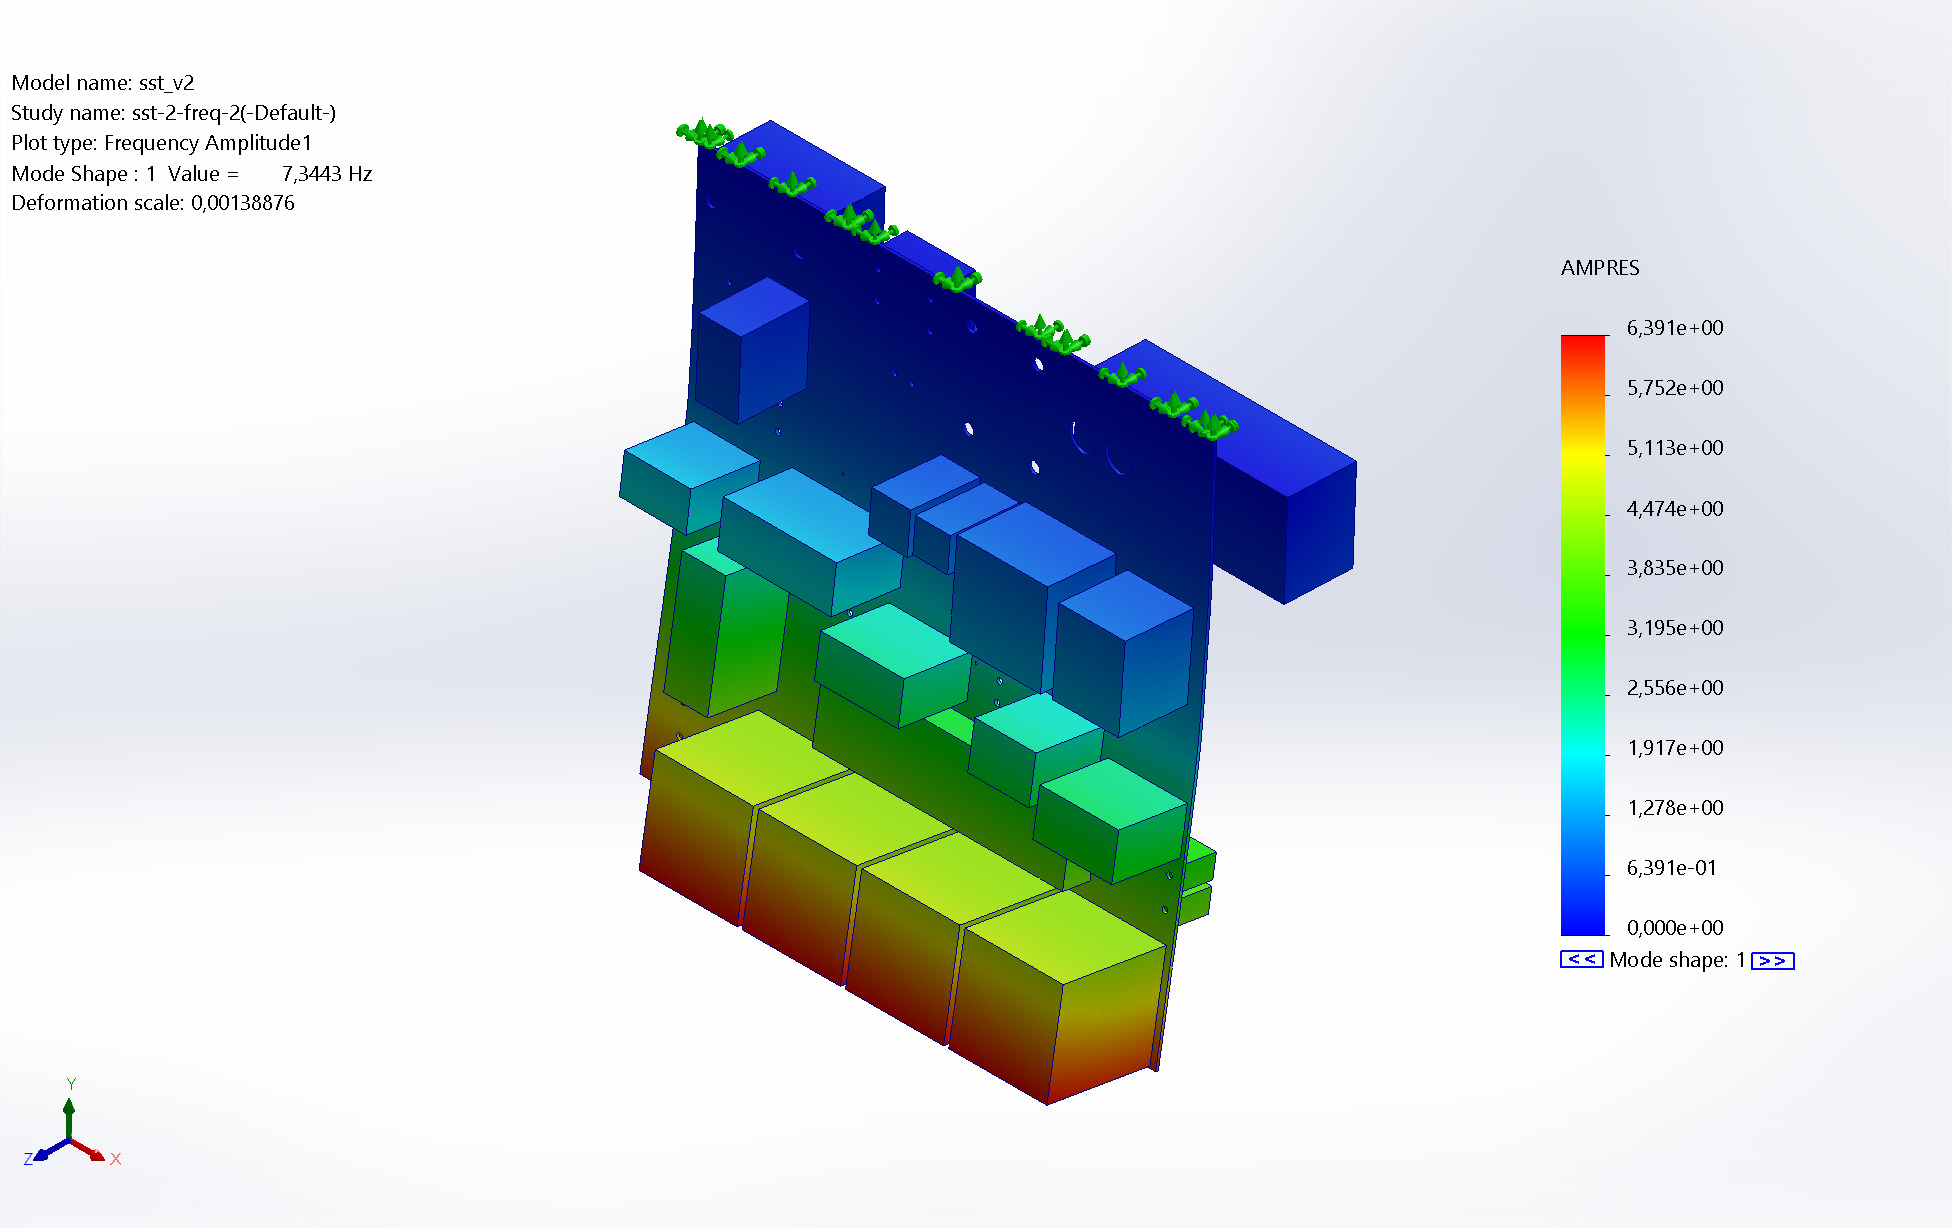
\includegraphics[scale = 0.3]{../img/sst-2/freq/sst_v2-sst-2-freq-2-Amplitude-Amplitude1.jpg}
  \caption{Результаты частотного анализа в \textit{SOLIDWORKS SIMULATION} второго варианта компоновки ПП.}

\end{figure}

На рисунке 10 представлены результаты частотного анализа в
\textit{SOLIDWORKS Simulation} третьего варианта компоновки печатной платы.


\begin{figure}[H]
  \centering
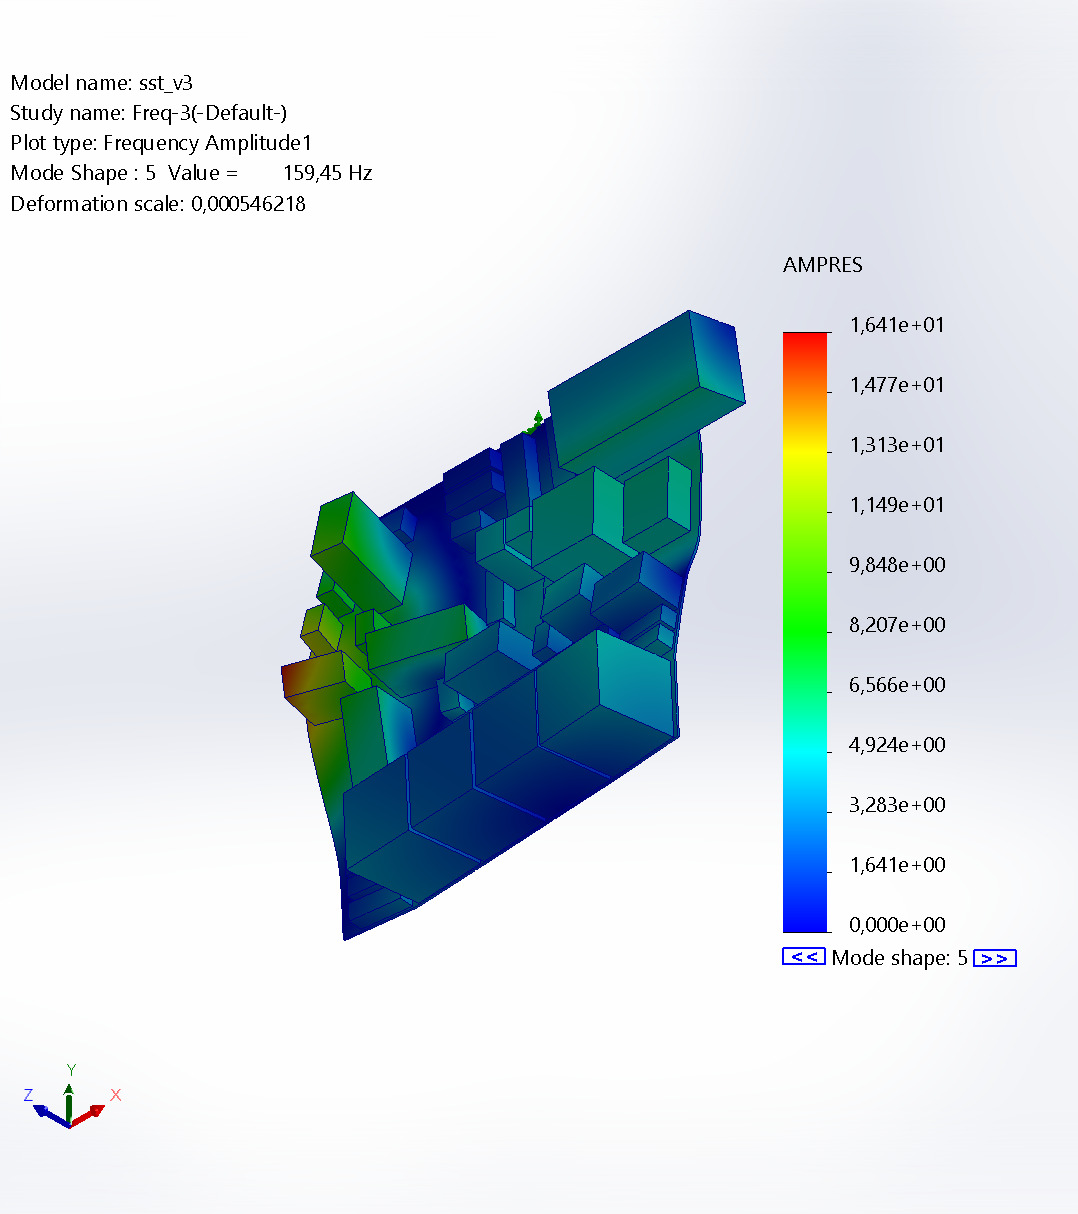
\includegraphics[scale=0.3]{../img/sst-3/freq/sst_v3-Freq-3-Amplitude-Amplitude1.jpg}
\caption{Результаты частотного анализа в \textit{SOLIDWORKS Simulation} третьего варианта компоновки ПП.}
\end{figure}

На рисунке 11 представлены результаты частотного анализа в
\textit{COMSOL Multiphysics} первого варианта компоновки печатной платы.

\begin{figure}[H]
  \centering
  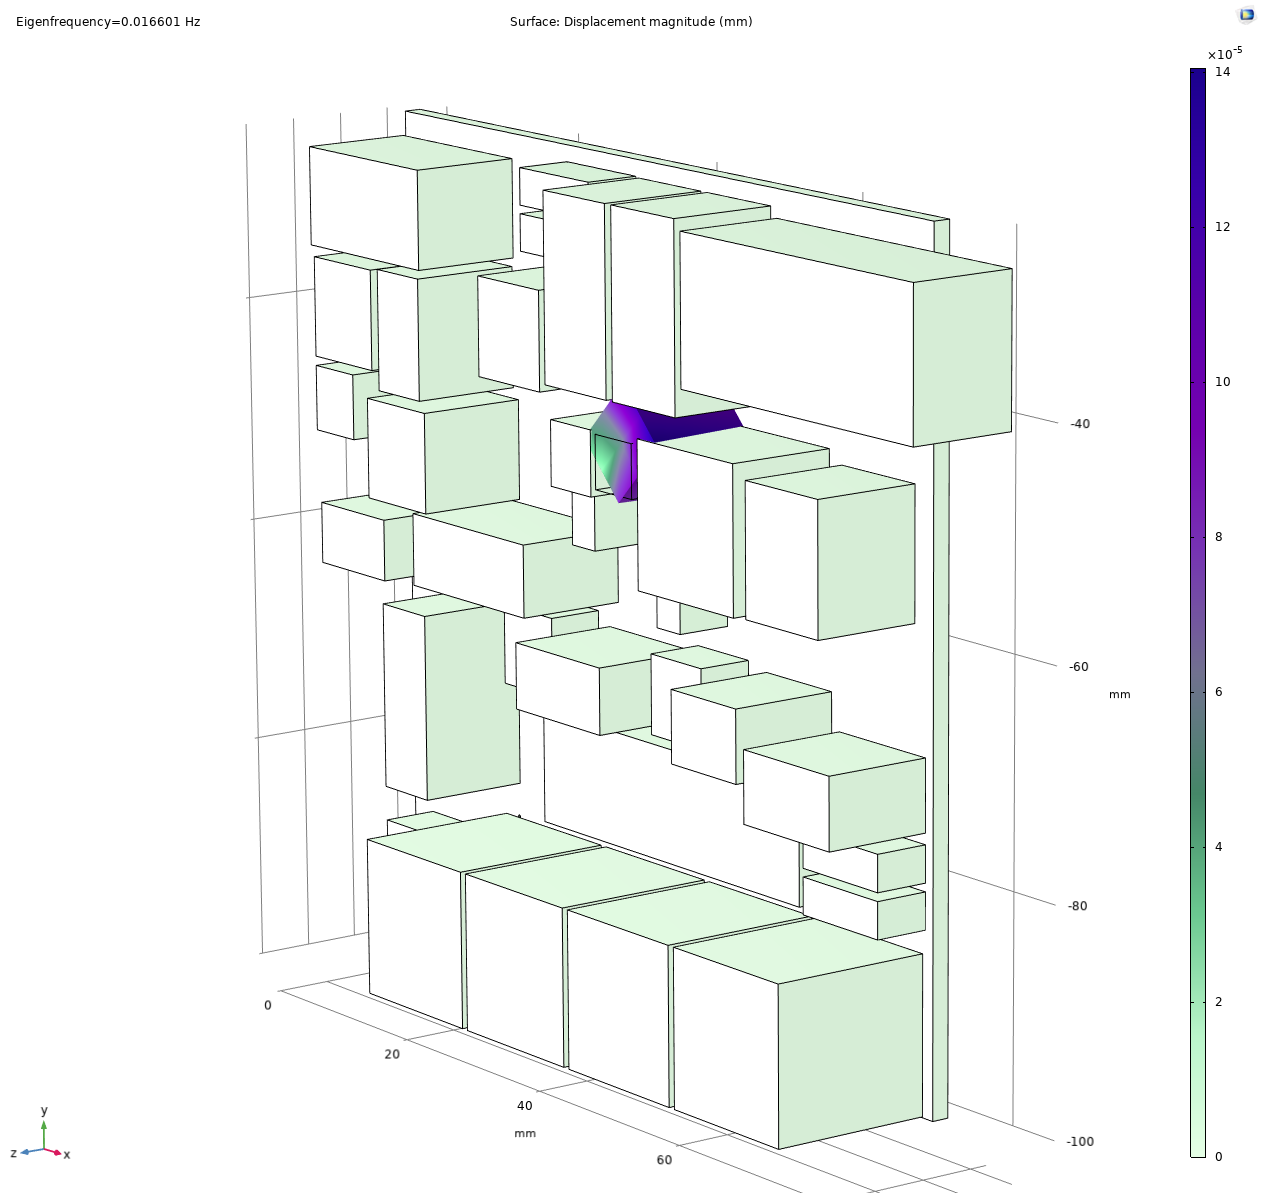
\includegraphics[scale=0.3]{../img/sst-1/freq/comsol.png}
  \caption{Результаты частотного анализа в \textit{COMSOL Multiphysics} первого варианта компоновки}
\end{figure}

На рисунке 12 представлены результаты частотного анализа в \textit{COMSOL Multiphysics} второго вараинта компоновки печатной платы.

\begin{figure}[H]
  \centering
  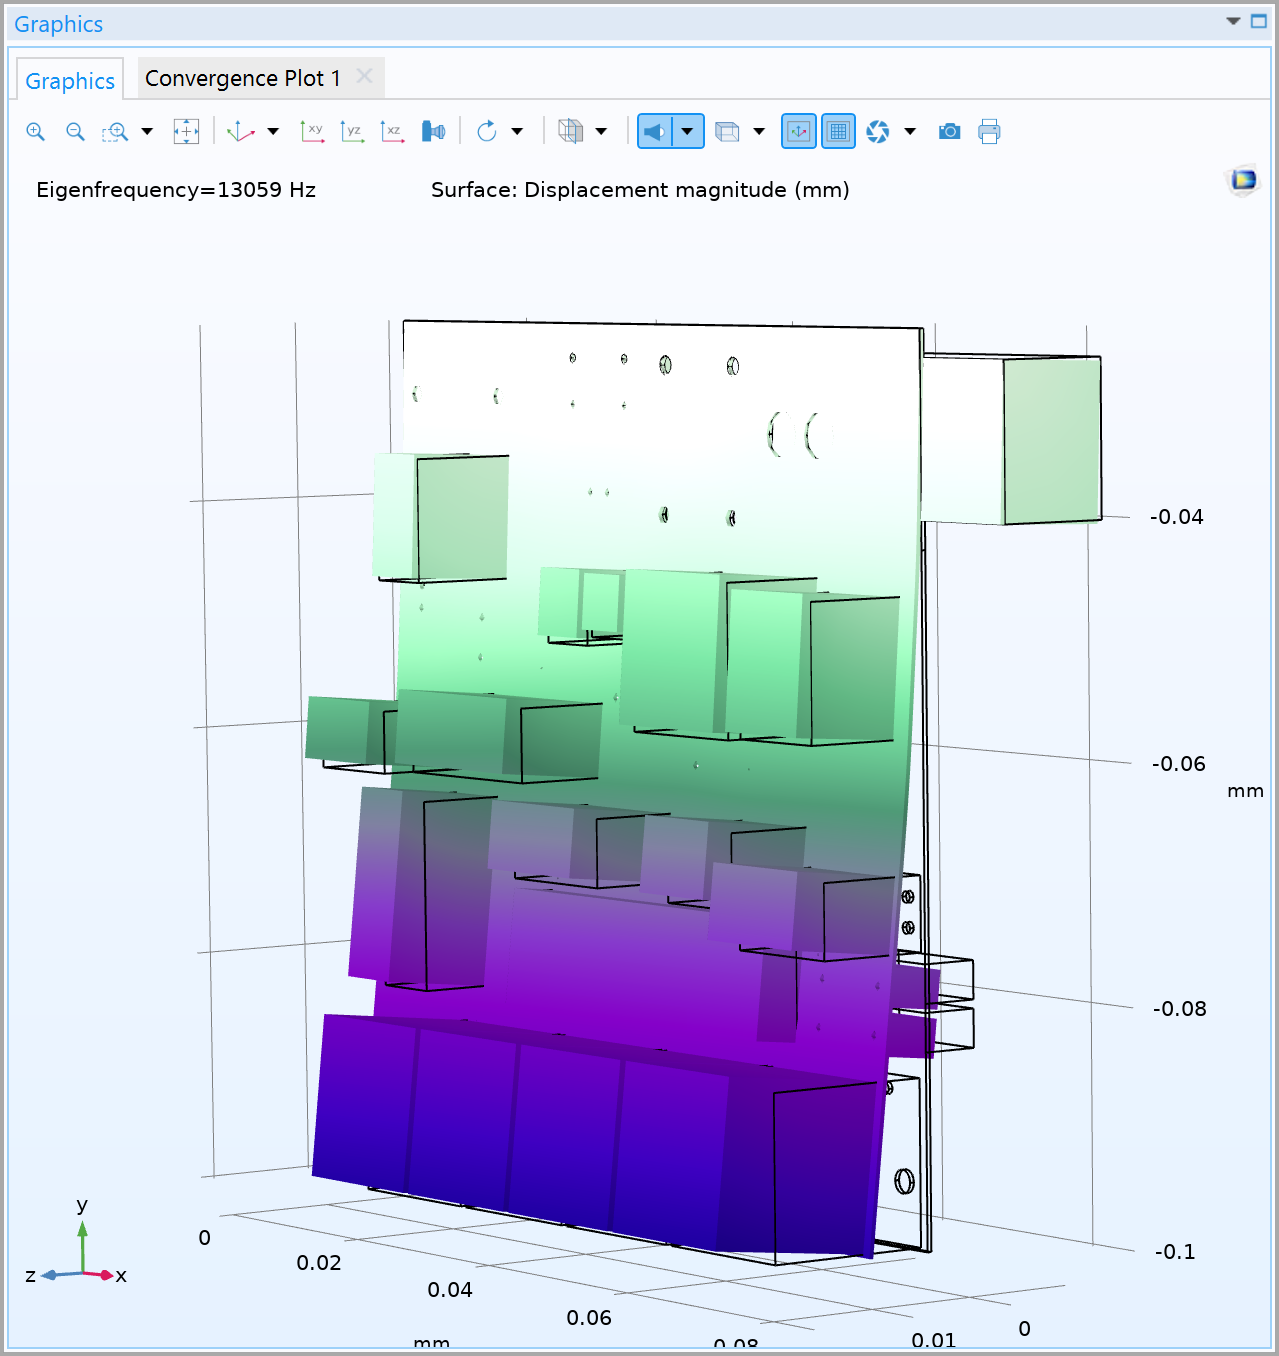
\includegraphics[scale=0.3]{../img/scrot/Screenshot-2024-05-16-014808.png}
  \caption{Результаты частотного анализа в \textit{COMSOL Multiphysics}
    второго варианта компоновки}
\end{figure}

На рисунке 13 представлены результаты частотного анализа в \textit{COMSOL Multiphysics} третьего варианта компоновки печатной платы.

\begin{figure}[H]
  \centering
  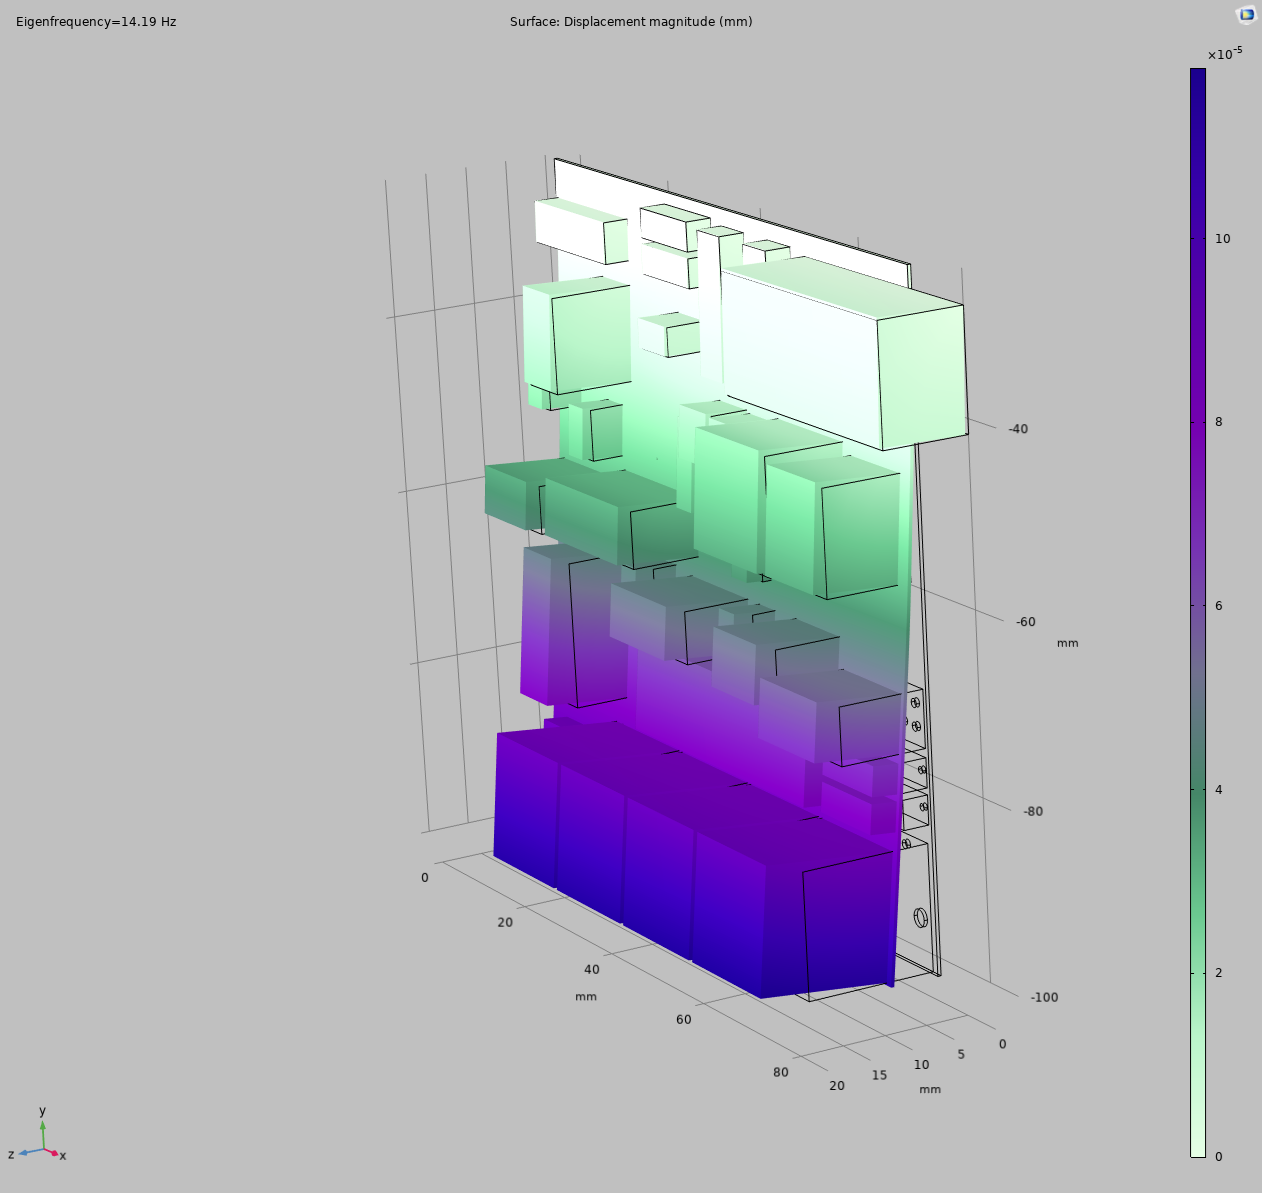
\includegraphics[scale=0.3]{../img/sst-3/freq/comsol.png}
  \caption{Результаты частотного анализа в \textit{COMSOL Multiphysics}
    третьего варианта компоновки}
\end{figure}
